\documentclass[14pt, a4paper]{article}
\usepackage[utf8]{inputenc}
\usepackage[russian]{babel}
\usepackage{multirow}
\usepackage{graphicx}

\title{\textbf{Отчет о выполнении лабораторной работы 1.4.5}}
\author{Калашников Михаил, Б03-205}
\date{}

\begin{document}

\maketitle

\textbf{Цель работы:} исследование зависимости частоты колебаний струны от величины натяжения, а также условий установления стоячей волны, получающейся в результате сложения волн, идущих в противоположных направлениях.

\begin{figure}[!h]
\centering
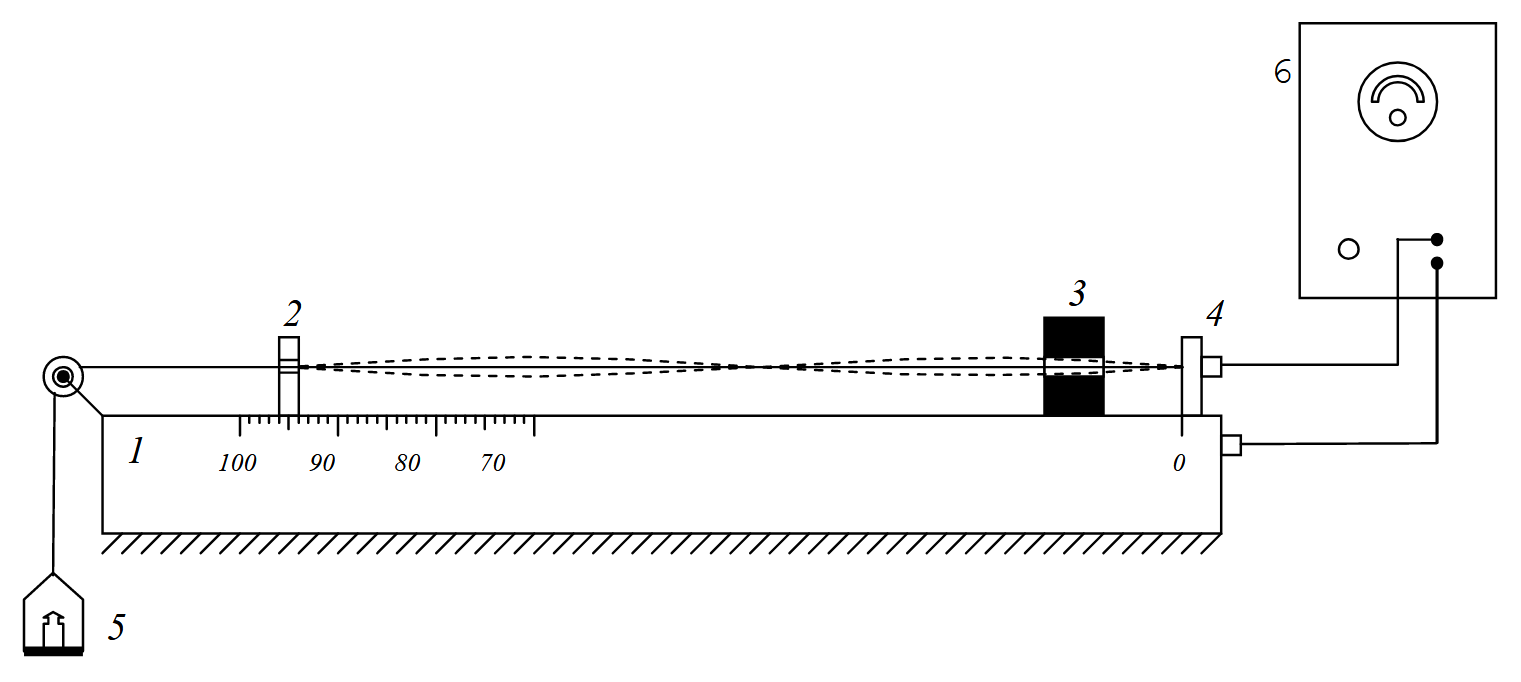
\includegraphics[scale=0.25]{laba7_setup.png}
\label{img_setup}
\caption{Схема установки}
\end{figure}

В лабораторной работе использовалась установка, схема которой представлена на рис. \ref{img_setup}. На массивной металлической рейке 1 установлены опора 2 и магнит 3, которые можно перемещать вдоль рейки, а также неподвижная опора 4. Один конец струны закреплен в изоляторе опоры 4. От него струна проходит между полюсами магнита и через опору 2, которая дает возможность струне перемещаться в горизонтальном направлении, неподвижный блок и соединяется с чашкой 5, на которую помещают грузы. Такое устройство необходимо для натяжения струны. К концу струны, закрепленному в изоляторе опоры 4, и к массивной металлической рейке 1 подводится переменное напряжение от звукового генератора 6. Движение струны вызывается силой Ампера, действующей на проводник с током в магнитном поле.
Постепенно нагружая чашу, будем находить частоты колебаний струны, при которых образуются стоячие волны. Опыт проведем с пятью разным нагрузками при повышении и понижении частоты сигнала генератора. Зафиксированные значения занесем в таблицу \ref{table_frq}.
\newpage

\begin{table}[!h]
\centering
\begin{tabular}{| c | c | c | c | c | c | c | c | c |}
\hline
\multirow{2}{*}{N} & \multirow{2}{*}{$m$, $g$} & $n$ & 1 & 2 & 3 & 4 & 5 & 6 \\
\cline{3-9}
& & \multicolumn{7}{| c |}{$\nu$, $Hz$} \\
\hline
\multirow{2}{*}{1} & \multirow{2}{*}{949.9} & $\Uparrow$ & 127 & 255 & 383 & 512 & 640 & 771 \\
\cline{3-9}
& & $\Downarrow$ & 127 & 255 & 383 & 511 & 640 & 771 \\
\hline
\multirow{2}{*}{2} & \multirow{2}{*}{1442.3} & $\Uparrow$ & 157 & 314 & 470 & 629 & 787 & 946 \\
\cline{3-9}
& & $\Downarrow$ & 156 & 314 & 471 & 629 & 787 & 946 \\
\hline
\multirow{2}{*}{3} & \multirow{2}{*}{1939.7} & $\Uparrow$ & 182 & 364 & 546 & 729 & 912 & 1096 \\
\cline{3-9}
& & $\Downarrow$ & 182 & 364 & 547 & 729 & 913 & 1096 \\
\hline
\multirow{2}{*}{4} & \multirow{2}{*}{2432.9} & $\Uparrow$ & 204 & 408 & 612 & 816 & 1021 & 1227 \\
\cline{3-9}
& & $\Downarrow$ & 203 & 407 & 611 & 816 & 1020 & 1225 \\
\hline
\multirow{2}{*}{5} & \multirow{2}{*}{2852.1} & $\Uparrow$ & 223 & 446 & 669 & 893 & 1117 & 1341 \\
\cline{3-9}
& & $\Downarrow$ & 222 & 445 & 669 & 892 & 1116 & 1340 \\
\hline
\end{tabular}
\label{table1}
\caption{Измерения частоты колебаний струны}
\end{table}

Частота $\nu_n$ связана с числом полуволн $n$ соотношением $\nu_n=n\frac{u}{2l}=nk_1.$ Выразим скорость распространения звука в струне $u$. Коэффициент $k_1$ найдем с помошью МНК, построив экспериментальную зависимость $\nu_n(n)$.
\[u=2lk_1, \sigma_u=u\sqrt{\left(\frac{\sigma_l}{l}\right)^{2}+\left(\frac{\sigma_{k_1}}{k_1}\right)^{2}}.\]

\begin{figure}[!h]
\centering
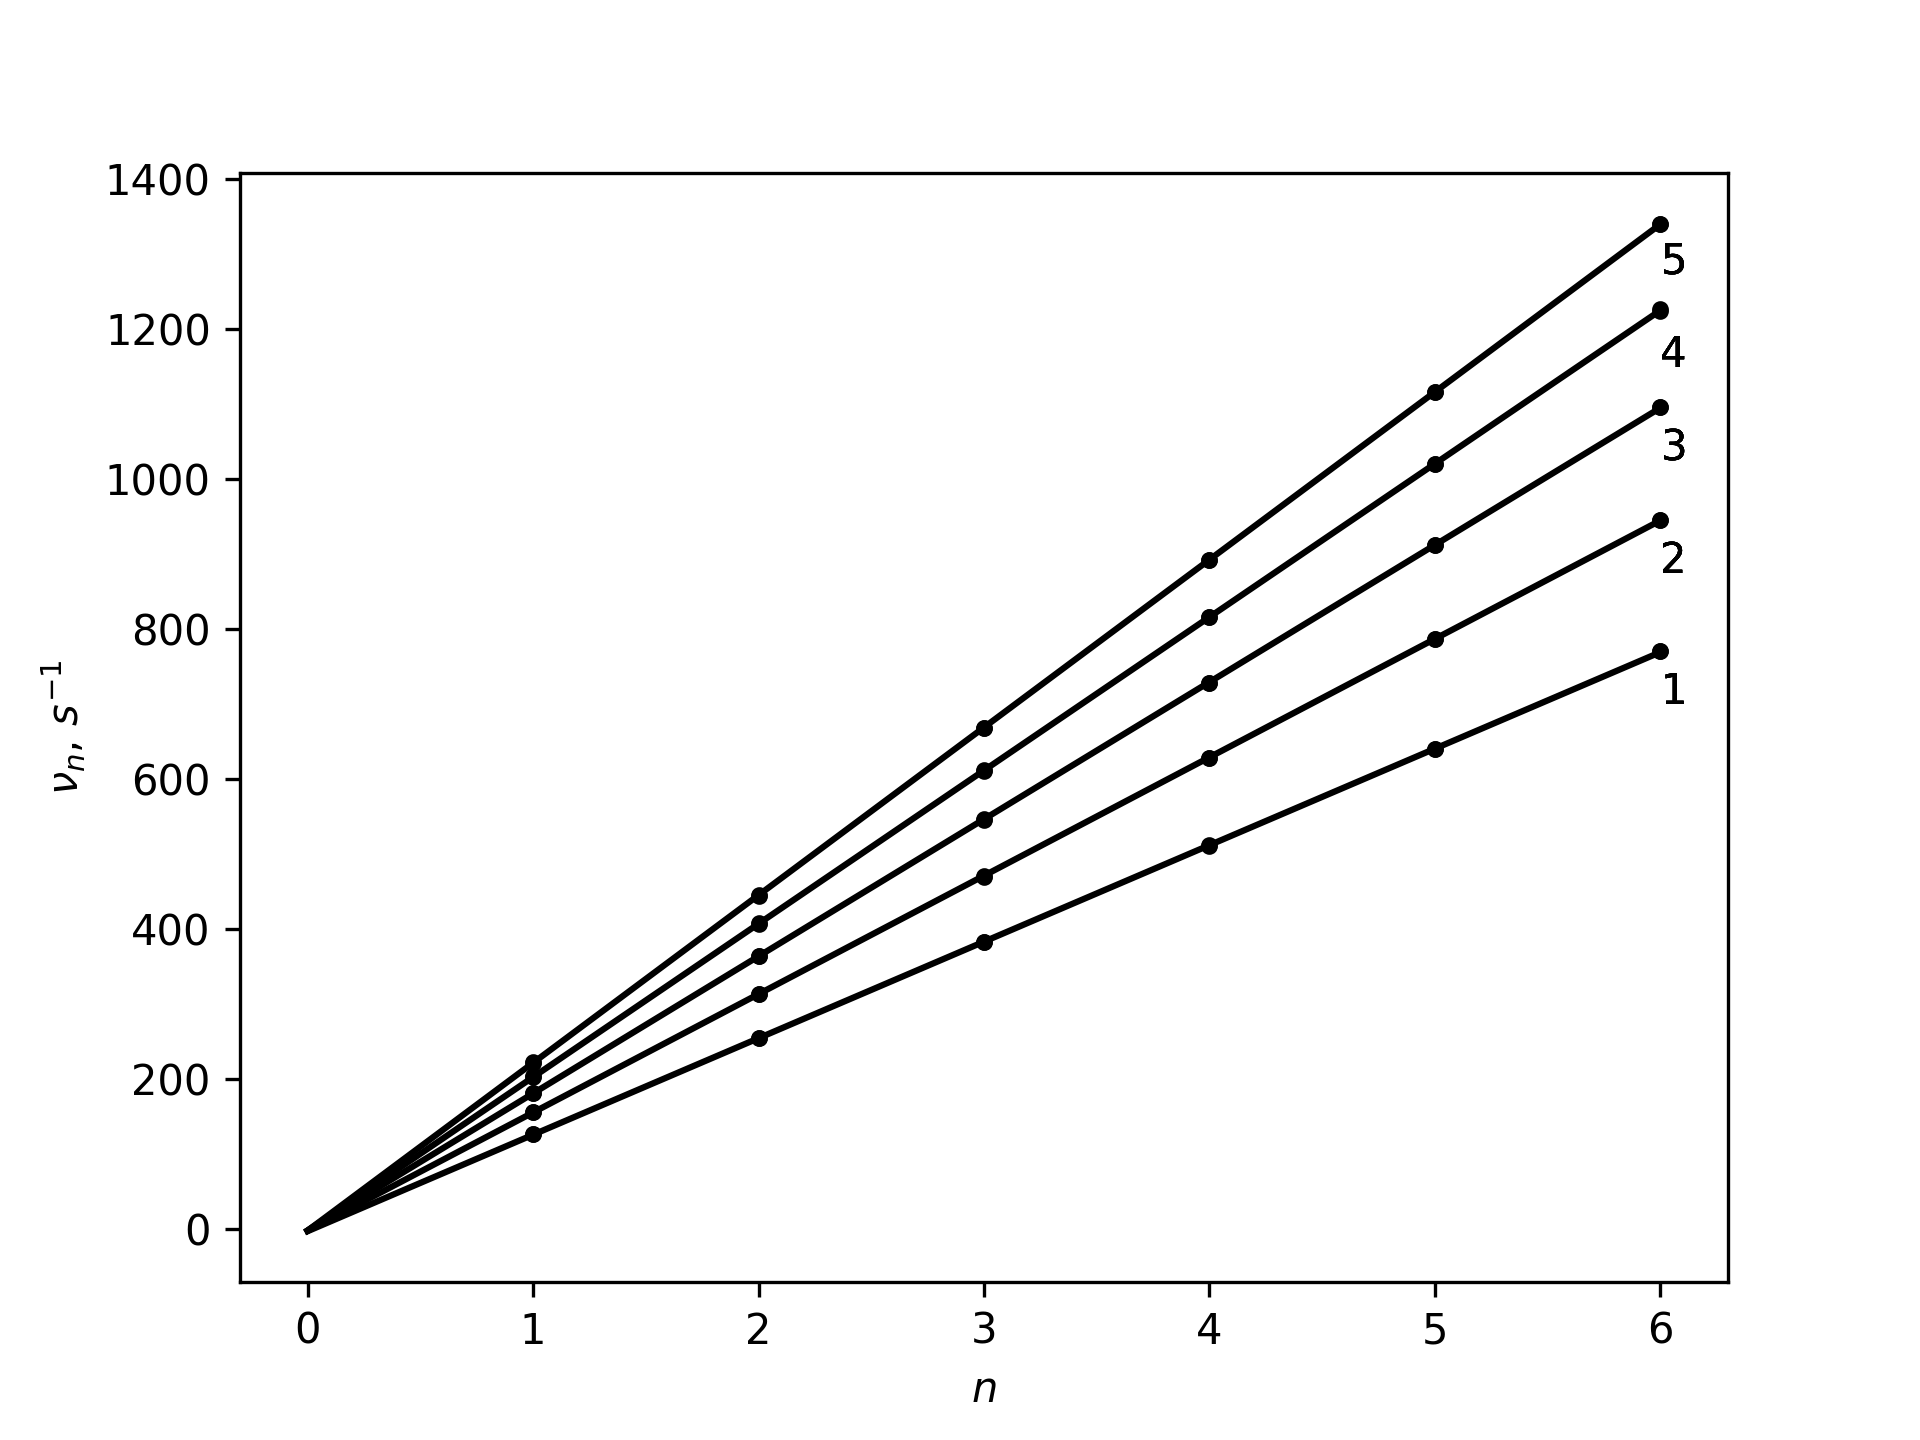
\includegraphics[scale=0.55]{laba7_1.png}
\caption{График зависимости $\nu_n(n)$}
\end{figure}

\begin{table}[!h]
\centering
\begin{tabular}{| c | c | c | c | c | c |}
\hline
$N$ & 1 & 2 & 3 & 4 & 5 \\
\hline
$m$, $g$ & 949.9 & 1442.3 & 1939.7 & 2432.9 & 2852.1 \\
\hline
$k_1$, $s^{-1}$ & $128.67\pm0.08$ & $157.86\pm0.08$ & $182.8\pm0.08$ & $204.46\pm0.08$ & $223.61\pm0.08$ \\
\hline
$u$, $m\cdot s^{-1}$ & $128.67\pm0.27$ & $157.86\pm0.33$ & $182.8\pm0.38$ & $204.46\pm0.42$ & $223.61\pm0.46$ \\
\hline
\end{tabular}
\caption{Вычисление скорости звука в струне}
\end{table}

\newpage

Аналогичным образом с помощью МНК может быть получен коэффициент $k_2$, связывающий квадрат скорости звука $u$ и массу нагрузки $m$. Построим график по точкам, которые мы получили ранее и проведем через них прямую. На основе коэффициента $k_2$ может быть рассчитана погонная плотность струны $\rho_l$.

\begin{figure}[!h]
\centering
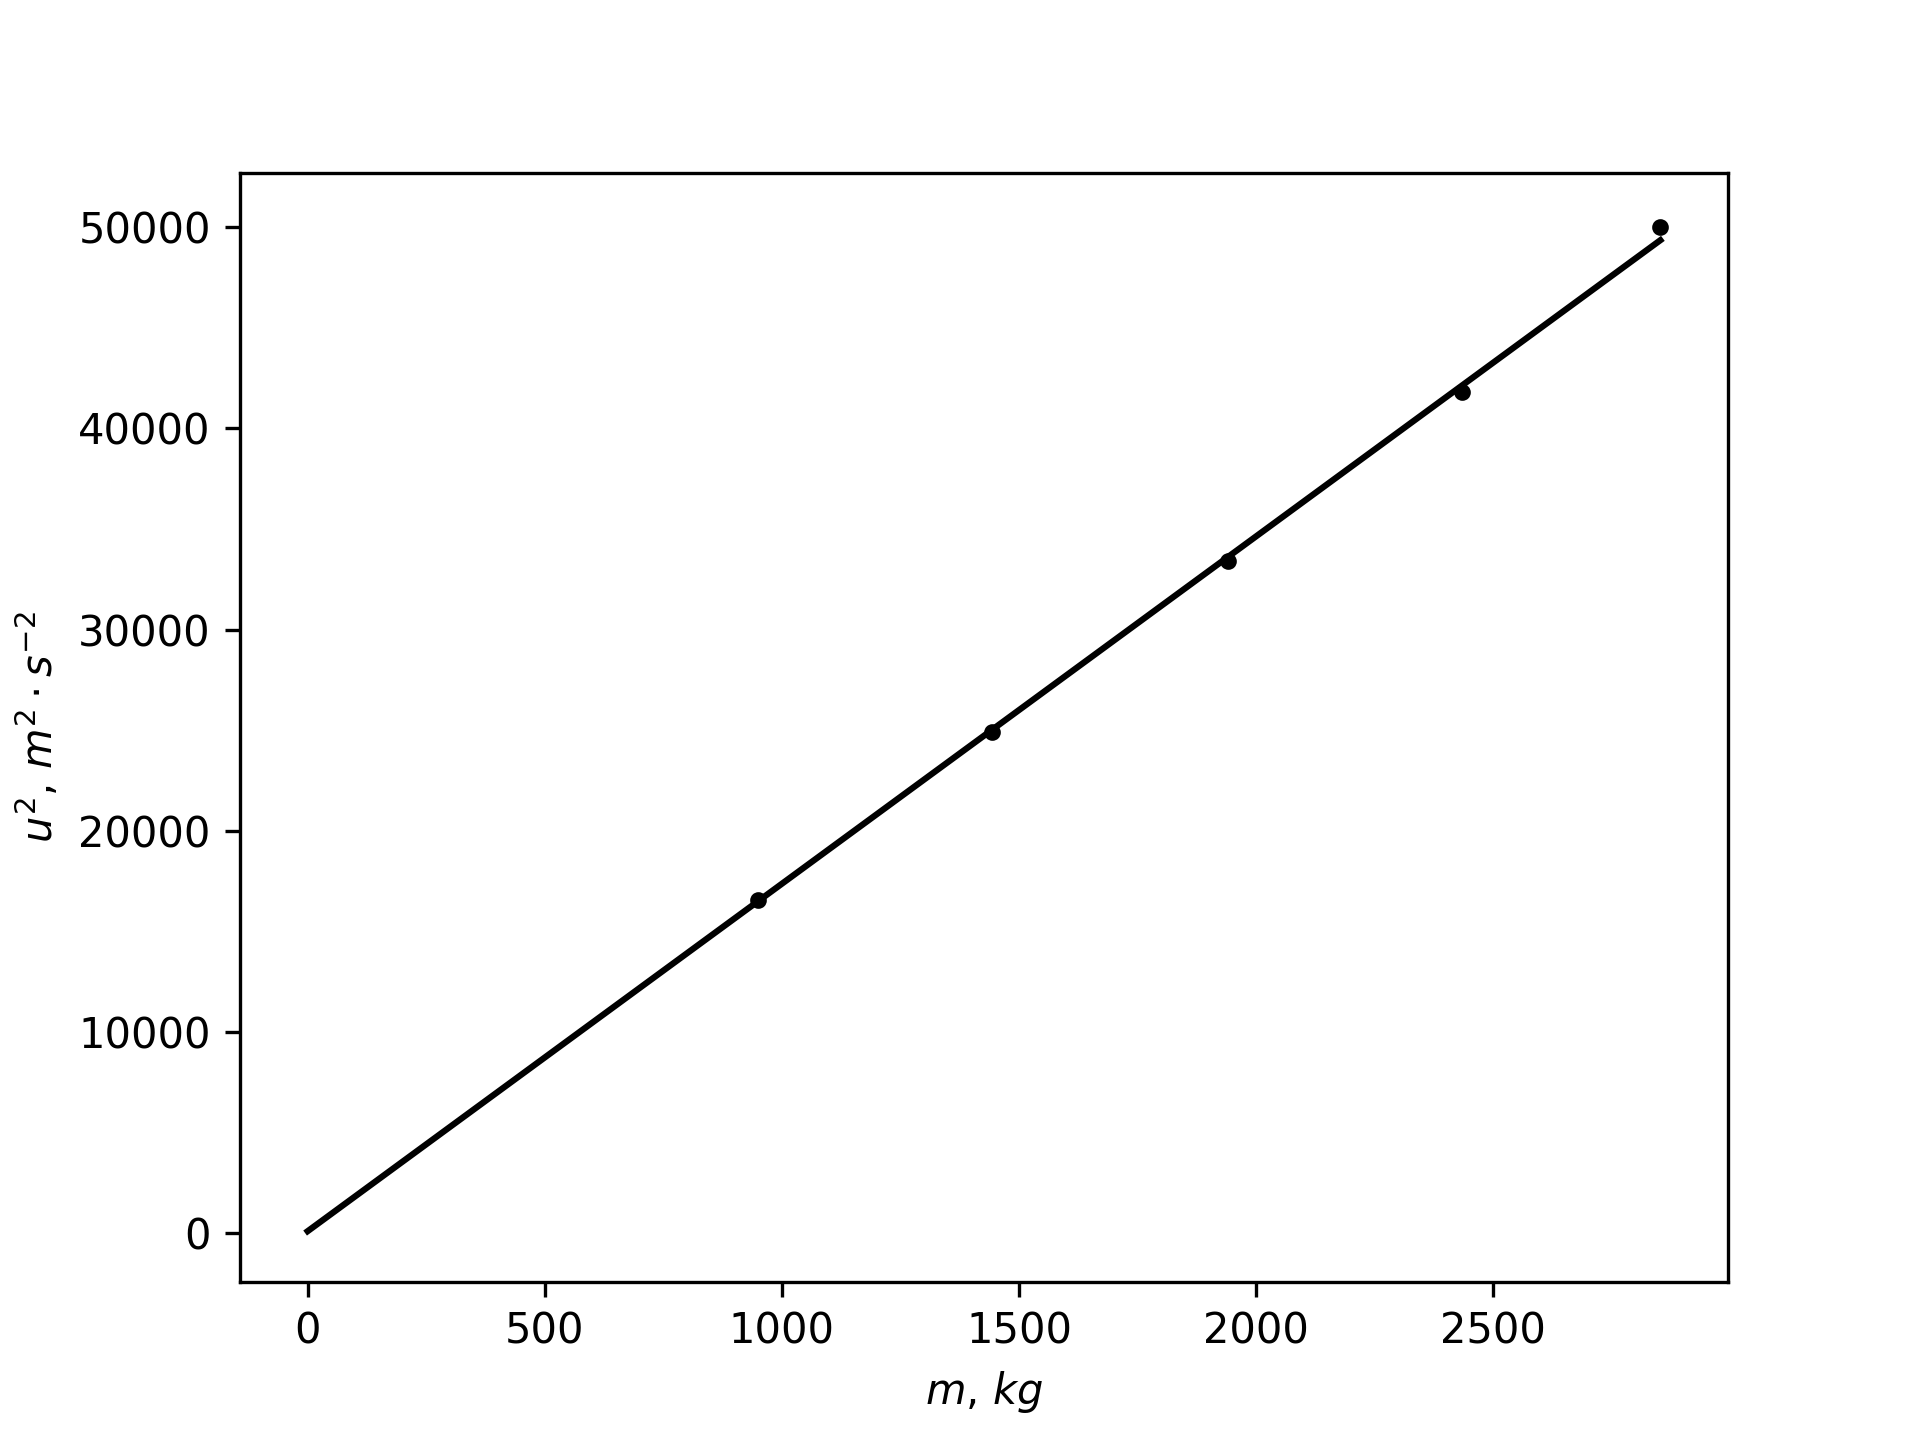
\includegraphics[scale=0.55]{laba7_2.png}
\caption{График зависимости $u^2(m)$}
\end{figure}

\[u^2=\frac{F}{\rho_l}=mk_2\]
\[k_2=17.28\pm0.08\ m^2s^{-2}g^{-1}\]

\[\rho_l=\frac{g}{k_2}, \sigma_{\rho_l}=\rho_l\frac{\sigma_{k_2}}{k_2}\]
\[\rho_l=568.06\pm2.73\ mg\cdot m^{-1}\]

Значение погонной плотности указанное на установке составляет 
\[\rho_{l0}=568.4\ mg\cdot m^{-1}.\]

\end{document}